\documentclass{getwriting}
\title{\lstinline{getwriting}: A Minimal~\LaTeX~Template For Journal Articles}
\author[1,2]{Notice the ORCID links, PhD \orcidlink{xxxx-xxxx-xxxx-xxxx} \thanks{firstauthor@famoustown.edu}}
\author[3]{Emails are in the footnote \orcidlink{xxxx-xxxx-xxxx-xxxx} \thanks{secondauthor@historytown.edu}}
\author[1,3]{Usually only this person's email needs to be shown, PhD \orcidlink{xxxx-xxxx-xxxx-xxxx} \thanks{thirdauthor@lessfamoustown.edu}}
%usually only the corresponding authors' emails are on the manuscript, but you can add all if you want
\affil[1]{\footnotesize Department of Science, University of Famoustown}
\affil[2]{\footnotesize Department of Mathematics, University of Lessfamoustown}
\affil[3]{\footnotesize Department of History, University of Historytown}
\begin{document}
\maketitle
\begin{abstract}
    This is an example of the document that can be generated with the \lstinline{getwriting} class. I usually use this template or minor variations thereof to write manuscripts.
    \par
    This class offers a quick start to writing articles by including commonly used packages and a template that matches the general format of most journal articles. I have kept available options to the bare minimum. If you really want to tweak something, edit the cls file. 
    \par
    This is a tidy, minimal, readable, \textit{good enough} format that has everything you need and nothing you don't. 
    \par
    \textbf{Don't waste time formatting your document, just start writing.}
    \par
    If you need to reformat your document for journals later, it's easy to copy and paste from this template as there are almost no custom sections.
    \\\\
    \textbf{Keywords:} Article templates, Overleaf, minimal, bioR$\chi$v, medR$\chi$v, format-free submissions,~\LaTeX
\end{abstract}
\section{Introduction}
\textbf{How to use this template: }Import all files in this repository into Overleaf (yes, Overleaf, since it has the best package manager and managing~\LaTeX~packages on a personal installation is a nightmare and \textbf{you should be writing}. Keep this tex file around for reference. Use a copy of this file to get started writing and fill in all the sections. \textbf{I used the XeLaTex compiler}. 
\par
This document uses the beautiful and free Atkinson Hyperlegible font, which is designed for low-vision readers. You should consider doing the same. The TrueType font files are included with this template and you can download the font from the Braille Institute here: \url{https://brailleinstitute.org/freefont}.
\par
Previous work has shown something, but not this, and I have cited a paper~\cite{scbonita}. 
\par
Look, this is a new paragraph. \textbf{And here is some bold text.} I can even \textit{italicize} text.
\par
I can refer to subsequent sections and elements like so: \hyperref[results]{\autoref{results}} and modify the display text like so: \hyperref[fig:figure1]{Look at figure 1!}.
\par
\subsection{Disclaimers}
This is a numbered subsection, by the way.
\par
\textbf{This template is provided as-is} and I take no responsibility for any errors/disasters. I'm not a~\LaTeX~expert even though I can typeset~\LaTeX~and I can even cite papers~\cite{scbonita} and cross-reference equations~\hyperref[eq:refname]{(\autoref{eq:refname})}. Play with the .cls file, look it up on StackOverflow and/or the Overleaf documentation, do whatever you like.
\section{Results}\label{results}
\subsection{Citations and cross-references}
Here are some magnificent results. Previous work has shown something, but not this, and I have cited a paper~\cite{scbonita}. 
\par
Here's how to cross-reference a table:~\hyperref[tab:table1]{\autoref{tab:table1}}
\par
Here is how I would typeset the name of a software package: \lstinline{software}
\subsection{All About Figures}
Here is even more data. I can reference a figure to support my point \hyperref[fig:figure1]{\autoref{fig:figure1}}.
You can find this figure in \hyperref[figures]{\autoref{figures}}. You can even refer to a supplementary figure: \hyperref[fig:supplementaryfigure1]{\autoref{fig:supplementaryfigure1}}. Note the difference in the figure title format. This is set by a renewcommand line in the \hyperref[suppinfo]{Supplementary Information section}.
\par
Speaking of figures, here are the rules for this minimal template. Most of these rules apply to tables as well apart from the ones that don't.
\begin{outline}
    \1 Figures must all be in a section at the end. Don't bother trying to have the figures near where you reference them. This is a futile, time- consuming exercise \& \textbf{you should be writing, not formatting}. Notice how I formatted the ampersand (\&).
    \1 Each figure must start on a new page. This is the only clean way.
\end{outline}

\section{Materials and Methods}
\section{How to Format}
\subsection{All About Text Formatting}
You should almost never highlight text, but here's how you can: \hl{this is a highlighted phrase}.\\
Consider \textit{italics}, \textbf{bold} or \emph{emphasis} instead.\\
Write inline math like this ($\sqrt{-1}$), Greek letters like this ($\alpha$), inline math and Greek together like this ($\alpha + \beta = \gamma$), and basic chemical formulae or any text requiring super/sub-scripts in math mode like this $O_2$, $O^2$, $O_{1,2,3}$. 
\subsection{All About Equations}
I can refer to equation eq:refname like so: this is some text about \hyperref[eq:refname]{\autoref{eq:refname}} and I can also modify display text in the hyperlink like this \hyperref[eq:refname]{(\autoref{eq:refname} This is a string)}
\begin{equation}
	\cos^3 \theta =\frac{1}{4}\cos\theta+\frac{3}{4}\cos 3\theta
	\label{eq:refname}
\end{equation}
\section{All About Lists}
I can list things like this:
\begin{enumerate}
	\item First item in a list
	\item Second item in a list
\end{enumerate}
Or even like this:
\begin{itemize}
	\item{First item in a list}
	\item{Second item in a list}
\end{itemize}
\textit{\textbf{But I really prefer \textbf{multi-level lists} like this:}}
I have pre-set the \lstinline{enumerate} package options to show Arabic numerals for level 1, lower-case alphabet for level 2, and lower-case Roman numerals for level 3. This is a sensible default and you're unlikely to gain much from changing them.
\begin{outline}[enumerate]
	\1 First item in an outline
	\2 Second item in an outline
	\3 Third item in an outline
	\1 Fourth item in an outline
	\2 Fifth item in an outline
\end{outline}
\section{Discussion}
All rules are meant to be broken (for good reasons). Use this template as just that, a \textit{template}. 
\par
\begin{center}
    \Large{\textit{\textbf{Happy writing!}}}
\end{center}
\newpage
\section{Figures}\label{figures}
\begin{figure}[H]
\label{fig:figure1}
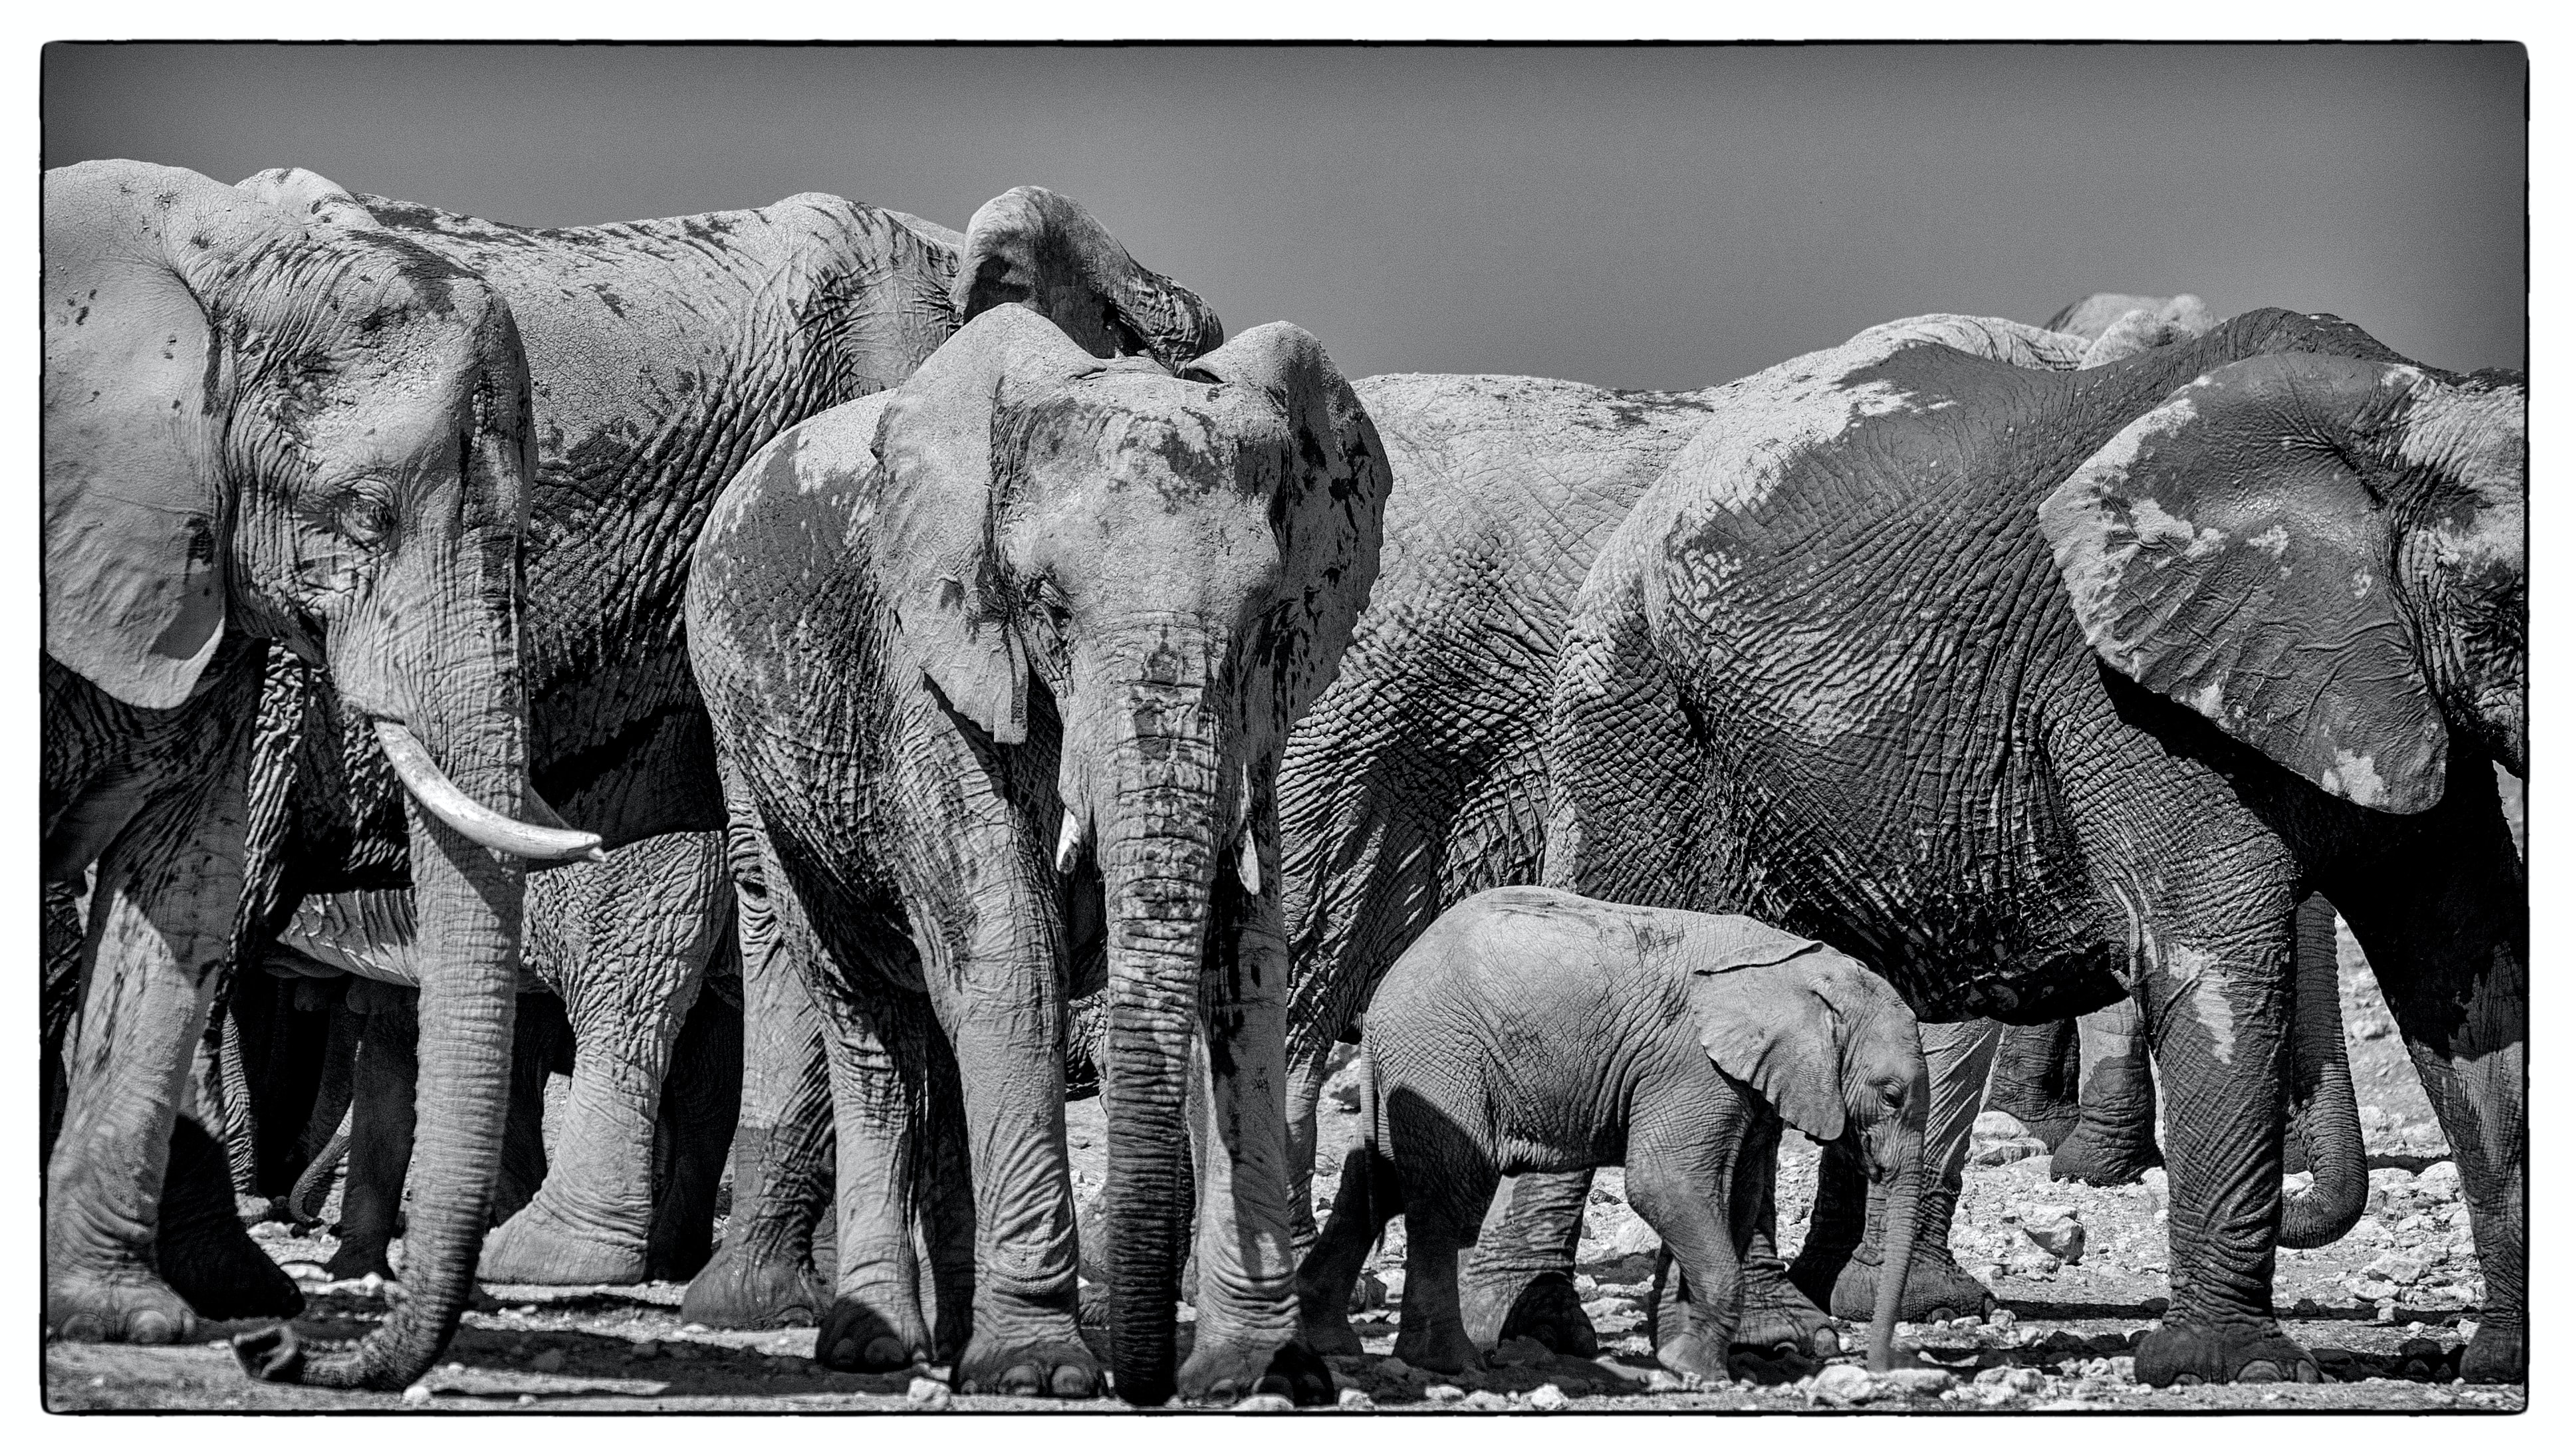
\includegraphics[width=5.25in]{figures/testPicture.jpg}
\caption{\textbf{Here is the title of my caption} Here is text describing each panel in this figure. This is a photograph by Bob Brewer and incidentally this is how you typeset a URL: \url{https://unsplash.com/photos/sFsumfD7Pbs}}
\end{figure}
\newpage
\section{Tables}
Rules for tables:
\begin{outline}
\1 Each table goes on a new page. All tables should be in this section.
\1 I only use the longtables and booktabs packages, regardless of the length of the tables. These produce beautiful and readable tables. It's easy to generate longtable code from a CSV with Pandas: \url{https://pandas.pydata.org/docs/reference/api/pandas.DataFrame.to_latex.html}
\1 The makecell command allows multi-lined cells.
\end{outline}
\par
An example table~\hyperref[tab:table1]{(\autoref{tab:table1})} will start on the next page.
\newpage
\begin{longtable}{lll}
\caption{Here's a table made with \lstinline{longtable} and \lstinline{booktabs}. This is the loooooong caption.}
\label{tab:table1}\\
\toprule
\makecell{\makecell{Column 1}} & \makecell{\makecell{Column 2}} & \makecell{\makecell{Column 3}} \\ \\
\midrule
\endfirsthead
\caption[]{This is the SHORT caption that is shown when a table continues to the next page} \\
\toprule
\makecell{\makecell{Column 1}} & \makecell{\makecell{Column 2}} & \makecell{\makecell{Column 3}} \\ \\
\midrule
\endhead
\midrule
\multicolumn{3}{r}{{Continued on next page}} \\
\midrule
\endfoot
\bottomrule
\endlastfoot
          \makecell{Row 1} &  \makecell{something} &  \makecell{anything}\\
          \makecell{Row 2} &   \makecell{something} &  \makecell{anything}\\
            \makecell{Row 3} &   \makecell{something} &  \makecell{anything}\\
                      \makecell{Row 1} &  \makecell{something} &  \makecell{anything}\\
          \makecell{Row 2} &   \makecell{something} &  \makecell{anything}\\
            \makecell{Row 3} &   \makecell{something} &  \makecell{anything}\\
                      \makecell{Row 1} &  \makecell{something} &  \makecell{anything}\\
          \makecell{Row 2} &   \makecell{something} &  \makecell{anything}\\
            \makecell{Row 3} &   \makecell{something} &  \makecell{anything}\\
                      \makecell{Row 1} &  \makecell{something} &  \makecell{anything}\\
          \makecell{Row 2} &   \makecell{something} &  \makecell{anything}\\
            \makecell{Row 3} &   \makecell{something} &  \makecell{anything}\\
                      \makecell{Row 1} &  \makecell{something} &  \makecell{anything}\\
          \makecell{Row 2} &   \makecell{something} &  \makecell{anything}\\
            \makecell{Row 3} &   \makecell{something} &  \makecell{anything}\\
                      \makecell{Row 1} &  \makecell{something} &  \makecell{anything}\\
          \makecell{Row 2} &   \makecell{something} &  \makecell{anything}\\
            \makecell{Row 3} &   \makecell{something} &  \makecell{anything}\\
                      \makecell{Row 1} &  \makecell{something} &  \makecell{anything}\\
          \makecell{Row 2} &   \makecell{something} &  \makecell{anything}\\
            \makecell{Row 3} &   \makecell{something} &  \makecell{anything}\\
                      \makecell{Row 1} &  \makecell{something} &  \makecell{anything}\\
          \makecell{Row 2} &   \makecell{something} &  \makecell{anything}\\
            \makecell{Row 3} &   \makecell{something} &  \makecell{anything}\\
                      \makecell{Row 1} &  \makecell{something} &  \makecell{anything}\\
          \makecell{Row 2} &   \makecell{something} &  \makecell{anything}\\
            \makecell{Row 3} &   \makecell{something} &  \makecell{anything}\\
\end{longtable}
\newpage
\section*{Funding}
Thanks for the money.
\section*{Acknowledgements}
Shoutout to all my friends. 
\section*{Abbreviations}
\textbf{HIV}: human immunodeficiency virus; \textbf{DNA}: deoxyribonucleic acid
\newpage
\section*{Supplementary Information}
\label{suppinfo}
Supplementary Information should start on a new page. \\
The redefinitions below will make sure that your supplementary figures and tables are referred to as 'Supplementary Figure X' and 'Supplementary Table Y' respectively.
\setcounter{figure}{0}    
\renewcommand{\figurename}{Supplementary Figure }
\makeatletter
\def\fnum@figure{\figurename\thefigure}
\makeatother
\renewcommand{\tablename}{Supplementary Table }
\newpage
\subsection*{Supplementary Figures}
\begin{figure}[H]
\label{fig:supplementaryfigure1}
\begin{center}
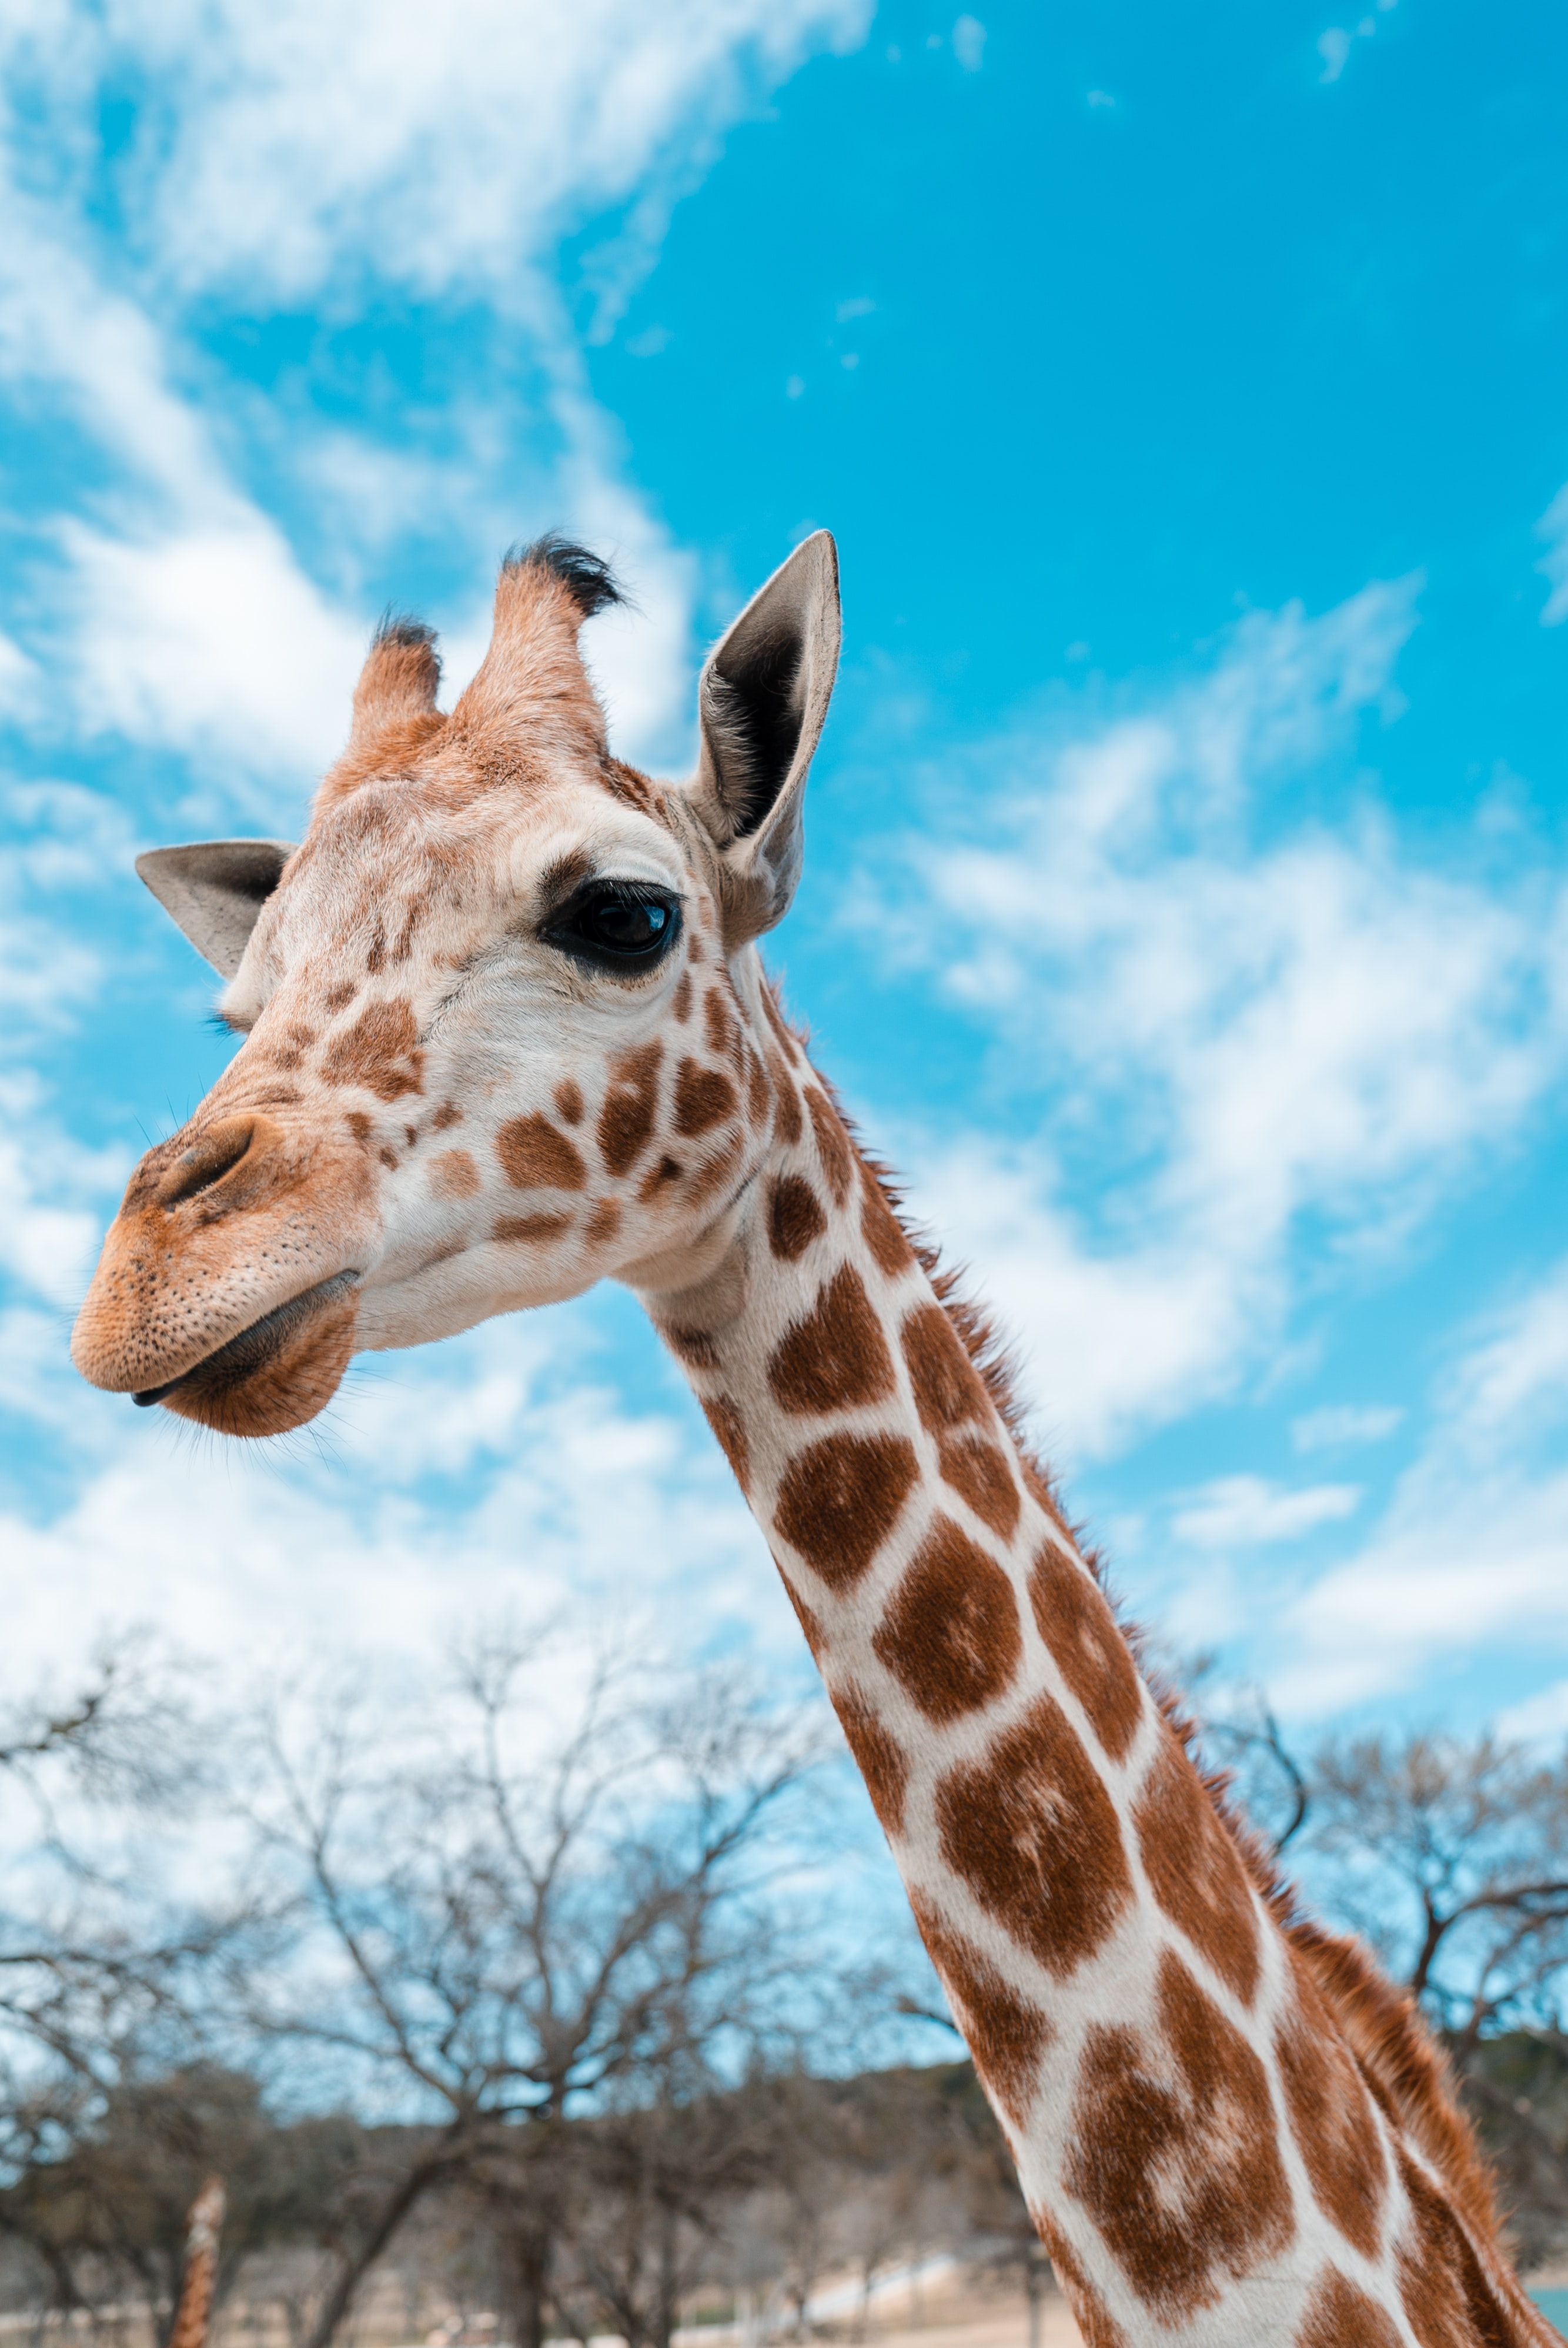
\includegraphics[width=3.25in]{figures/supplementaryTest.jpg}
\end{center}
\caption{\textbf{Here is a VERTICAL figure that I have CENTERED.} Here is text describing each panel in this figure. This is a photograph by Andreas Dress and you can find the original here: \url{https://unsplash.com/photos/NNe6epzHGm8}}
\end{figure}
\newpage
\subsection*{Supplementary Tables}
Add some tables here.
\newpage
\bibliography{getwriting}
\end{document}
